\section{Experiments}\label{sec:expts}

% TODO: needs to show comparison of no. iterations required for optimizing using LBFGS vs. without gradient. Or compare performance after 20 iterations of each.

\begin{table}
\begin{tabularx}{\textwidth}{| p{1.9cm} | X | X | X | X | X | X | X | X |}
\hline
Dataset & Folds /subs-amples & Users & Items & Pairs, train & Pairs, test & Pref vals, test & Item features & User features \\
\hline\hline
Simulation (a) & 25 & 25 & 100 & 900 & 0  & 100 & 2 & 2\\
Simulation (b) & 25 & 25 & 100 & 900 & 0 & 100 & 2 & 2 \\
Simulation (c) & 25 & 25 & 100 & 900 & 0 & 100 & 2 & 2\\
Simulation (d) & 25 & 25 & 100 & 36 - 2304 & 0 & 100 & 2 & 2\\
\hline
Sushi A & 25 & 1000 & 10 & 15000 & 5000 & 10000 & 18 & 123 \\
Sushi B & 25 & 5000 & 100 & 50000 & 5000 & 500000 &  18 & 123 \\
\hline
UKPConvArg-CrowdSample & 32 & 1442 & 1052 & 16398 & 529 & 33 & 32310 & 0
\\ \hline
\end{tabularx}
\caption{Summary of datasets showing mean counts per subsample or per fold. For the simulation datasets, generate the subsamples of data independently, for the Sushi dataset we select subsamples independently from the complete dataset, while  
UKPConvArgCrowdSample is divided into folds, where the test data in each fold corresponds to a single topic and stance. The numbers of features are given after categorical labels have been converted to one-hot encoding, counting
each category as a separate feature.
}
\label{tab:datasets}
\end{table}
% NOTE: possible problem with convincingness data is that some users have very few observations in training data.
We use the datasets summarized in Table \ref{tab:datasets} to test the key aspects of our proposed methods: recovering an underlying consensus from noisy pairwise labels; modeling personal preferences from pairwise labels; and the scalability of our proposed Bayesian preference learning methods, GPPL and crowd-GPPL using SVI.
In Section \ref{sec:exp_synth}, we use simulated data to test the ability of our method to recover preference functions from noisy data when the correct number of latent factors is unknown. 
Section \ref{sec:exp_scale} evaluates our approach on an NLP task with high-dimensional feature vectors and
a larger number of items, which involves using pairwise judgments of arguments from online debate forums 
to learn a function of argument \emph{convincingness}. We use the \emph{UKPConvArgSample},
which is
sampled from data provided by ~\citet{habernal2016argument} dataset.
This section first analyzes the scalability of our SVI approach, then its performance in 
predicting preferences. 
Finally, in Section \ref{sec:sushi}, we compare our method against previous approaches for predicting the preferences
of thousands of users on the \emph{Sushi} datasets~\citep{kamishima2003nantonac}.

\subsection{Methods Compared}

We refer to the multi-user variant of our model as \emph{crowd-GPPL}.
As baselines, we use GPPL to learn a single preference function from all users' preference labels, (\emph{pooled-GPPL}), and a Gaussian process over the joint feature space of users and items 
(\emph{joint-GPPL}), as proposed by \citet{guo2010gaussian}.
For datasets up to 100 users (simulated data, subsamples of the real datasets), 
we also test separate GPPL instances per user with no collaborative
learning (\emph{GPPL-per-user}), but this could not be applied to the real datasets as the 
computation costs were too high.
To test the benefit of using GPs to model item and user features,
we also test two further baselines: 
\emph{crowd-GPPL$\mathbf{\setminus \bs u}$}, which ignores the user features,
and \emph{crowd-BMF}, which ignores both user and item features and so does not use GPs at all. 
For both of these methods, the user covariance matrix, $\bs K_w$, in the crowd-GPPL model is replaced by the identity matrix, and for \emph{crowd-BMF}, the item covariance matrices, $\bs K_v$ and $\bs K_t$ are also replaced by the identity matrix.

% Ranking-SVM baseline -- only easy to compare in the single user case. My GPPL paper perhaps needs
% this adding in any follow up works.

% Houlsby tests: with/without user features (without is better with few users). + a hierarchical 
% model, BI (multi task preference learning, Birlitiu et al), and the GPPL-joint model. None of 
% these are done at scale, which we can do with our inference method --> *this is a new claim i.e. 
% new empirical results*. They also test a per-user model.

\subsection{Simulated Noisy Data}\label{sec:exp_synth}

First, we test how well GPPL is able to recover an underlying consensus function
in the presence of varying amounts of noise.

We generate data by first selecting $100$ points at random
from a $10x10$ 2-dimensional grid and choosing $500$ pairs of these points at random. 
We generate pairwise labels by drawing from the single user GPPL model:
first, draw latent preference function values for the selected points; 
then, compute the pairwise likelihoods for the selected pairs using Equation \ref{eq:plphi};
draw pairwise labels from the Bernoulli likelihoods. 
We split the chosen points into 50\% training and test sets, and
train GPPL on all pairs involving only points in the training set.
We then use GPPL to latent predict preference function for the points in the test set.
We repeat this process, varying the value of $s$ in the generation step, 
which controls the precision of a latent preference function: as $s$ is increased, the latent
function values have a smaller amplitude and the pairwise labels become noisier.
The hyper-parameters of the GPPL model for prediction remain the same throughout, 
with $\alpha_0 = 2$, $\beta_0 = 2$.
We repeat the complete experiment $25$ times, including generating new data for each value of $s$.

The results of the first test in Figure \ref{fig:simA} show that increasing
the noise rate in the pairwise labels causes a near-linear decrease in the
rank correlation between the predicted and true preference function values. 
Nonetheless, GPPL is able to recover the ranking of points with $\tau > 0.5$ when
more than $1/3$ pairwise labels are incorrect.

In the second simulation, we recover a consensus function
from preference labels produced by multiple simulated users with varying differences
in their individual preferences. We use the same process as the first simulation, except
we now draw the pairwise labels from a crowd-GPPL model with $25$ users and $3$ latent factors,
instead of a single-user model. We fix the inverse scale of the latent item factors, $s=0.001$,
but vary the precision of the consensus function, $\sigma$. 
We use three methods to recover the consensus function, GPPL-per-user, pooled-GPPL, 
and crowd-GPPL with $C=25$ so that there is one factor per user. 
Figure \ref{fig:simB} shows that the crowd-GPPL model is better able recover the latent consensus
function than the other methods, even when noise levels are high. 
The pooled model's predictions may be worsened by biased users whose preferences deviate
 consistently from the consensus. GPPL-per-user relies on separate instances of GPPL, so 
 does not benefit from sharing information between users when training the model.

The third test repeats a similar setup to the second, but here we evaluate the methods'
ability to to recover the personal preferences of individual simulated users.
We fix $\sigma = 10$ and vary the precision of the item latent factors, $s$.
Results for predicting personal preferences in the presence of noise are shown in 
Figure \ref{fig:simC}. Crowd-GPPL is able to make better predictions when noise is below
$0.3$ but its benefit disappears when the noise level increases further. 

In the final simulation, we evaluate the effect of the quantity of training data 
in scenarios with different numbers of latent factors.
We hypothesized that a larger number of latent factors would indicate a more complex
scenario that would require more training data. 
We generate data again from the crowd-GPPL model with $s=0.2$ and $\sigma=1$
and vary the number of true latent factors using values $C_{true} \in \{ 1, 3, 10, 20\}$.
For each value of $C_{true}$, we run crowd-GPPL with increasing numbers of pairwise labels,
and evaluate the correlation between inferred and true latent user factors. 
To match inferred factors to true factors, we compute Pearson correlations between each
true factor and each inferred factor, then repeatedly select the pair of unmatched 
factors with the highest correlation as a new match until all true factors are matched. 

The results in Figure \ref{fig:simD} show that for all values of $C_{true}$, increasing the
number of training labels beyond $1000$ does not increase the correlations between the best-matched
latent user factors, and in fact the correlations decrease. Since the crowd-GPPL model
is able to learn $C=25$ factors, it may learn a more complex model that makes
more use of a greater number of latent factors given more training data.
In this case, the correlations may decrease as the true factors would be modeled by
multiple inferred factors, rather than just the best match. 
This may also explain why the correlations are higher when $C_{true} = 20$, as the
number of true factors is much closer to $C$. However, even when there is a large difference 
between $C_{true}$ and $C$, 
the correlation remains above 0.4, showing that the model is able to infer reasonable 
latent factors even when $C$ is set too high. 
% Does this pose a question: does the mismatch affect the performance? If the correlations
% decrease, it may mean that the model is decomposing a factor into a sum of multiple factors,
% or it may just be unable to learn it. This would need a new experiment: for 700 training pairs,
% how does the accuracy of personalised predictions vary with the number of latent factors?
% I think this needs us to vary C and keep C_true=3, otherwise we don't know whether the 
% performance differences are due to the mismatched no. factors or due to different underlying dataset, i.e. we need to keep the data the same to compare!
\begin{figure}
\subfloat[Inferring preferences for a single user]{
\label{fig:simA}
\includegraphics[width=.35\columnwidth]{../../results/synth_3/single_user/tau_test}
}
\subfloat[Inferring consensus function from crowdsourced labels]{
\label{fig:simB}
\includegraphics[width=.35\columnwidth]{../../results/synth_sandbox/multi_user_consensus/tau_test}
} \\
\subfloat[Inferring personal preferences for members of a crowd]{
\label{fig:simC}
\includegraphics[width=.4\columnwidth]{../../results/synth_sandbox/multi_user_personal/tau_test}
}
\subfloat[Inferring the latent factors]{
\label{fig:simD}
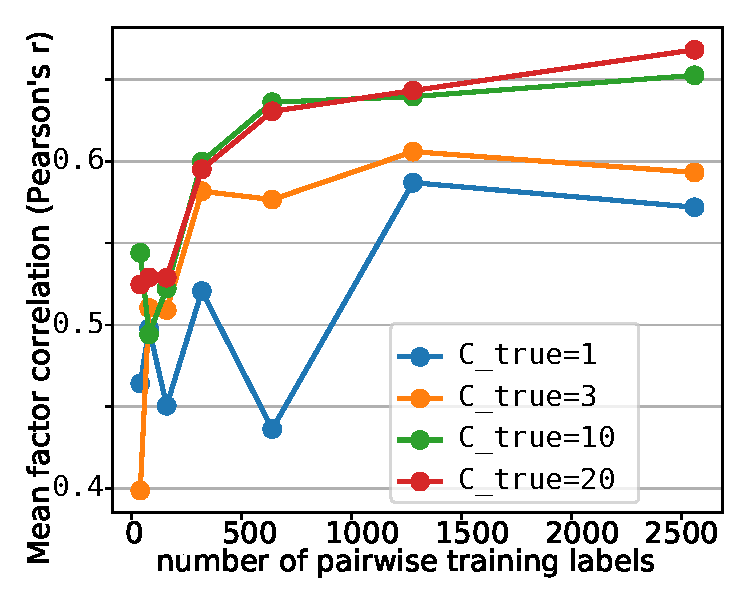
\includegraphics[width=.35\columnwidth]{../../results/synth_3/multi_factor_correlations_P/num_pairs_r}
}
\caption{Rank correlation between true and inferred preference values for different inference tasks.  (a)--(c) varying level of noise in pairwise training labels, (d) varying number of pairwise training labels. 
}
\end{figure}


\subsection{Argument Convincingness: Scalability}\label{sec:exp_scale}

We evaluate our preference learning approaches on an NLP dataset 
containing $32,310$ different features for arguments written by users
of online debating forums~\citet{habernal2016argument}.
The task is to quantify how convincing each argument is
by learning a model from pairwise preference labels obtained from crowdworkers
on Amazon Mechanical Turk. The workers were presented with pairs of arguments 
and asked to choose which argument was more convincing. 
The dataset is divided into $32$ parts, each corresponding to one of
$16$ topics and one of two opposing stances. 
We test the ability of the preference learning methods to predict the consensus
 by training on raw crowdsourced pairwise labels
for $31$ topics, and testing against the gold pairwise labels and rankings for the
remaining topic. This process is repeated for all $32$ topics.
This dataset, \emph{UKPConvArgCrowdSample}, was obtained in ~\citep{simpson2018finding}
by subsampling the raw crowdsourced labels provided by ~\citep{habernal2016argument},
and using the gold pairwise labels and rankings obtained in ~\citep{habernal2016argument}.

We assess our proposed SVI inference method by testing pooled-GPPL and crowd-GPPL with
different numbers of inducing points, $M$. Figure \ref{fig:M} shows the trade-off between
runtime and accuracy as an effect of choosing $M$. Accuracy close to the peak is attained
using $M=200$, after which the accuracy levels off, while the runtime increases rapidly
as $M$ increases.
With $300$ features, the polynomial training time complexity is visible in the runtime. 
However, with $33,210$ features, the runtime plot appears almost linear, since 
the cost of computing covariance matrices, which is linear in the number of features,
dominates the runtimes. The plots show that the SVI method provides a substantial cut
in runtimes while maintaining good prediction accuracy.

Figure \ref{fig:Ntr}, we compare the training + prediction runtimes of different methods as a
function of the training set size, $N_tr$. With a fixed $M$, runtimes increase very little 
with $N_tr$, as other overheads are inexpensive. The methods labeled "no SVI" show runtimes
for pooled-GPPL and crowd-GPPL with variational inference but no stochastic updates 
or inducing points. These are compared with Bi-LSTM and SVM classifiers trained to 
output probabilities of pairwise labels. The plots clearly show the rapid increases
in runtimes for these alternative methods. 
In Figure \ref{fig:Nfeatures}, we plot the number of features against runtimes for
each method on the whole dataset, with $M=500$. For pooled-GPPL and crowd-GPPL, 
the cost of kernel computations becomes visible only with $33,210$ features, 
indicating the benefits of more compact representations. BiLSTM appears unaffected by
additional input dimensions, while the SVM runtimes increase noticably from $30$ to $300$ and $3000$ features.

The pooled-GPPL method was previously tested on \emph{UKPConvArgCrowdSample}
in ~\citep{simpson2018finding}, and shown to outperform SVM, Bi-LSTM and Gaussian process classifier
methods. 
In this paper, we compare pooled-GPPL with crowd-GPPL and also test each method's 
ability to predict the raw crowdsourced labels, i.e. the individual preference labels
supplied by each worker.
We hypothesize that this task is subjective a worker's view of convincingness 
depends somewhat on their prior beliefs and understanding of the subject 
discussed and the language used. 
If this is the case, then provided that the data is sufficiently informative,
the crowd-GPPL model may more accurately predict unseen 
pairwise labels or rankings for individual workers,
and may be better able to predict the consensus preference function by accounting 
for the biases of individual workers.

% List of experiments to include -- need new plots for the crowd model:
% \begin{enumerate}
% \item Performance, computation time vs. no. inducing points
% \item Computation time vs. dataset size, no. features
% %\item not done: memory vs no. inducing points, update size
% %\item not done: Performance, computation time, vs update size
% %%\item not done: performance, computation time vs different initialisation methods for the inducing points; include different initialisations of K-means
% \end{enumerate}

% SCALABILITY ----------------------------------------------------------
\begin{figure}
\subfloat[Varying number of items in training set. GloVe features.]{
\label{fig:Ntr}
%    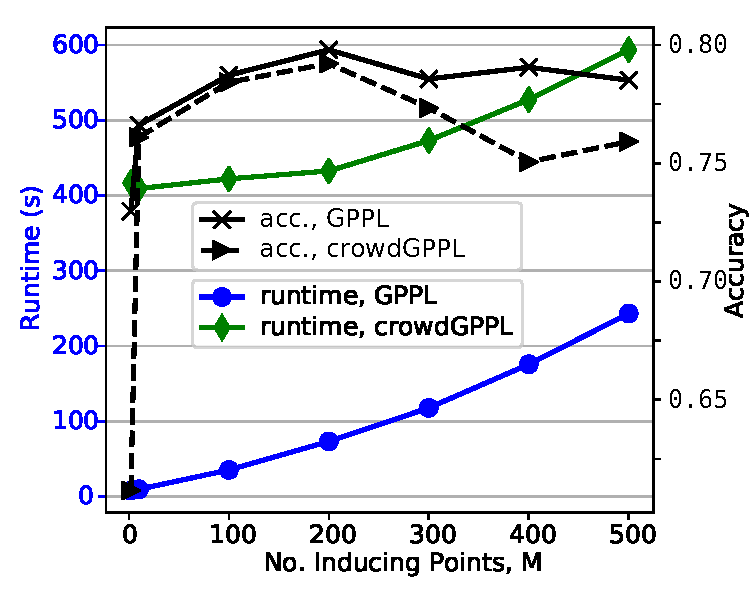
\includegraphics[width=.35\columnwidth]{../../results/scalability/num_inducing_32310_features}
}
\subfloat[Varying no. ling+GloVe features. $M=500$]{
\label{fig:Nfeatures}
 %   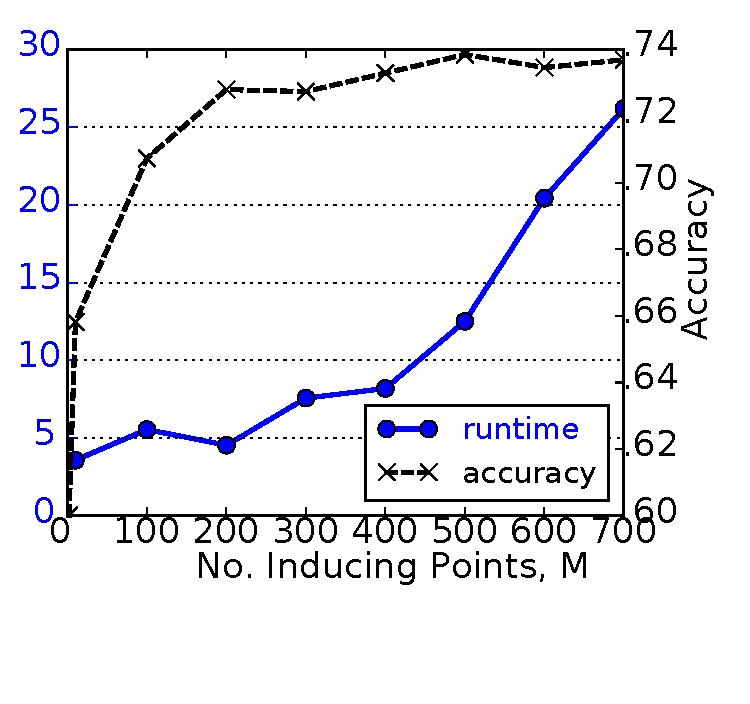
\includegraphics[width=.35\columnwidth]{../../results/scalability/num_inducing_300_features}
}
\caption{
    Runtimes for training+prediction on UKPConvArgCrowdSample with varying subsample size. Means over 32 runs. 
    Note the logarithmic x-axis for (b).
}
\end{figure}
\begin{figure}
\subfloat[300 GloVe features]{
 %   \includegraphics[width=.35\columnwidth]{../../results/scalability/num_features}
}
\subfloat[33210 ling+GloVe features]{
%    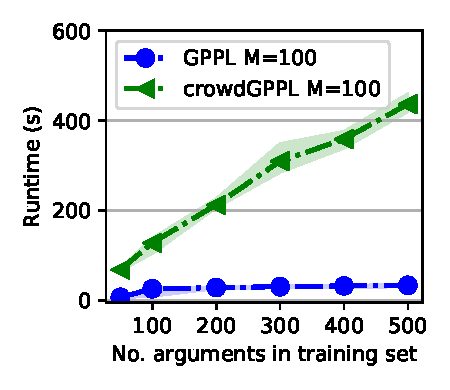
\includegraphics[width=.35\columnwidth]{../../results/scalability/num_arguments}
}
\caption{
Effect of varying $M$ on accuracy and runtime (training+prediction) for GPPL and crowd-GPPL on UKPConvArgCrowdSample. Means over 32 runs.
}
\label{fig:M}
\end{figure}

% PERFORMANCE ----------------------------------------------------

% TODO: exclude tau from the personal column -- not enough data to compute the gold standard correctly, only pairwise labels are real gold!

% Things we could do:
% forget about trying to predict the crowd consensus, focus on scalability
% This means we don't need to show performance improvements against 
% Houlsby or for crowd-gppl for the consensus prediction.

% however, if we want to show that the optimization procedure has improved performance, we should find out why the consensus results for crowd-GPPL are so bad. 
% It may be a data matchup error.

% Change to a different dataset instead of convincingness, or make sure to exclude workers with < 10 labels.

% For sushi, we can test on unseen users. This wasn't done by Khan or Houlsby. I guess
% that performance will be close to the pooled model, but it may help. This would
% demonstrate a benefit of the GP method.

\begin{table}
\begin{tabularx}{\columnwidth}{ | l | X | X | X | X | X | X |}
\hline
 & \multicolumn{3}{|X|}{Consensus}&\multicolumn{3}{| X |}{Personal} \\ \hline
 Method & Acc & CEE & Kend. & Acc & CEE & Kend. \\ \hline
 %SVM & .70 & .58 & .31 & .63 & .66 & .31 \\
 %Bi-LSTM & .73 &  .55 & .21 & .64 & .64 & .21 \\
 GPPL medi. & \textbf{.77} & \textbf{.50} &  \textbf{.40} & .71 & .56 & .07 \\
 GPPL opt. & & & & .70 & .58 &  .06 \\
 Crowd-GPPL medi. & .51 & .69 & .01 & .71 & .69 & .06 \\
 Crowd-GPPL opt. & .51 & .69 & .01 & .70 & .69 & .06
 %PL+ SVR & .75 & .55 & \textbf{.40} & .75 & & .40 \\
 %GPC & .73 & .53 & - & .68 & .59 & - \\
 \\\hline
\end{tabularx}
\caption{Performance comparison on UKPConvArgCrowdSample using ling+GloVe features. \emph{Acc} and \emph{CEE} show classification accuracy and cross entropy error (or log-loss) for pairwise predictions, 
while \emph{Kend.} shows Kendall's tau for the predicted preference function.}
\label{tab:convarg}
\end{table}
The performance metrics are shown in Table \ref{tab:convarg}....

We investigate whether how many latent factors were actively used by the crowd-GPPL model
by plotting the inferred variance scales, $s_c$, for the latent item factors in 
Figure \ref{fig:latent_factor_variance}. The plots show
that many factors have a very small variance and therefore do not contribute strongly 
to the model's predictions. This indicates that our Bayesian approach, in which the priors
of the latent factors have mean zero, preferred a simpler model even when a larger number
of latent factors was available.
\begin{figure}
\subfloat[UKPConvArgCrowdSample]{
%\includegraphics[width=.35\columnwidth]{../../results/conv_factors/UKPConvArgCrowdSample_factor_scales.pdf}
}
\subfloat[Sushi-A and Sushi-B]{
%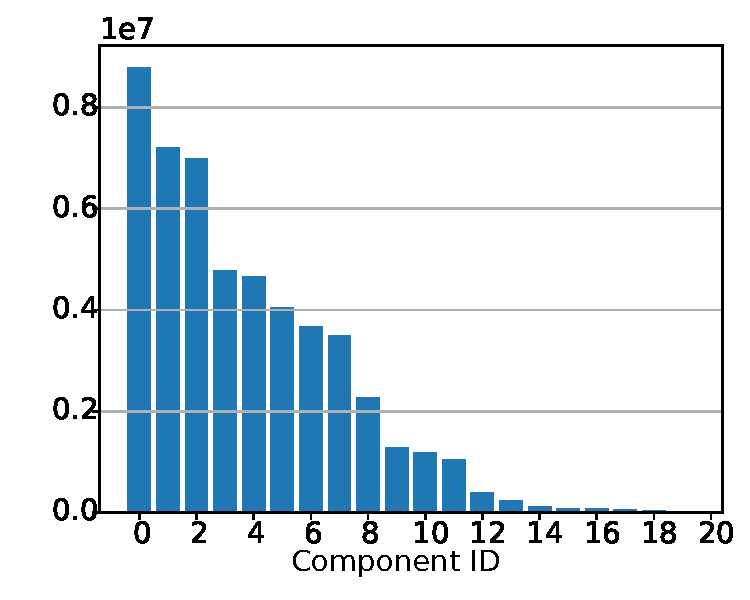
\includegraphics[width=.35\columnwidth]{../../results/sushi_factors/sushi_factor_scales}
}
\caption{
Distribution of latent factor variances, $1/s_c$, for crowd-GPPL on UKPConvArgCrowdSample, Sushi-A and Sushi-B, averaged over all runs.
}
\label{fig:latent_factor_variance}
\end{figure}

\subsection{Sushi Preferences}\label{sec:sushi}

We use two datasets, Sushi-A and Sushi-B (shown in Table \ref{tab:datasets}),
to benchmark the classification and ranking performance of GPPL and crowd-GPPL, 
as well as their runtimes, against previous approaches, 
and investigate the use of user features for predicting preferences.
The datasets contain, for each user, a gold standard preference ranking of $10$ types of sushi,
from which we generate pairwise labels. These labels can be considered noise-free, since
they are derived directly from the gold standard ranking.  
For Sushi-A, we select a subset of $1000$ workers at random, then 
split the data into training and test sets by randomly
selecting $15$ pairs for each user for training and $5$ for testing. 
For Sushi-B, we use all $5000$ workers, and subsample $10$ training pairs and $1$ test pair
per user.
We evaluate the quality of pairwise predictions using classification accuracy and cross entropy 
error (also known as log loss) to gauge the quality of the probabilities that each method outputs.
We also evaluate each method's inferred personal preference values
against the gold standard rankings by computing Kendall's $\tau$ rank correlation
coefficient between the negative rank and the inferred preference function values,
for all the items contained in each subsampled user's ranking.
The complete process, including subsampling, was repeated $25$ times.

% Houlsby results: for comparison against a different inference technique on small data, include
% the test error results from their paper.
% Guo results: not directly comparable. We will rerun a similar approach but with our inference method.
% Khan results: for a different model that separates the latent features from the item/user features.
% Abbasnejad results (community-based preference learning): sushi data with 10 items; 60/40 train/test split of each user's preference pairs. This means the result is based on 27 pairs training.
% don't worry about this though, it doesn't seem to work very well in their results.

% Number of users affects value of including user features.
% Plot results on increasing dataset size.

% [10] T. Kamishima. Nantonac collaborative filtering:
% Recommendation based on order responses. In
% ACM SIGKDD 9th Int. Conf. Knowledge Discov-
% ery and Data Mining, 2003.

% Run 25 repeats of random train/test splits with:
% Exclude these two as we focus on bigger datasets in this paper. Cutting these creates the space 
% for including three metrics.
% Downside: cannot test whether increasing no. users imroves performance through better collaborative learning. 
% 
% 100 (a la Houlsby 20 pairs per user), 
% 200 (a la Khan, 3 training, 1 test, P=600, P_test=200), 
% For small datasets, we may want to test on the argumentation data so we can assess the crowd
% consensus results with small data. That dataset is more interesting here because lots of items,
% small data is a new scenario.
% % % % [a] 1000 (a la Houlsby 15 training, 5 test pairs per user, $P=15000,P_{test}=5000$), Sushi-A (10 items), 
% % % % and [b] 5000 users (a la Khan, 10 training, 1 test pairs per user, $P=50000, P_{test}=5000$), Sushi-B (100 items).
% % % % Evaluate on parwise labelling error, pairwise label logloss, spearman rank correlation,
% % % % and runtime.
% could use normalized mean loss from guo, but not sure where the utilities come from -- ranking?

% 25 random train/test splits on all 5000 users with varying no. (1, 5, 10, 20, 40) pairs per user.

% Can put in the Houlsby (100/1000 users, 20 pairs each, labelling error) and Khan (200 users, 3 pairs each, logloss) results.
% Khan also provide code, so could be rerun to get classification error.


\begin{table}
\begin{tabularx}{\textwidth}{| l | X | X | X | l | X | X | X | l |}
\hline
& \multicolumn{4}{|c|}{\textbf{Sushi-A}} & \multicolumn{4}{c|}{\textbf{Sushi-B}} \\ 
Method & Acc. & CEE & Kend. & Runtime & Acc. & CEE & Kend. & Runtime \\
\hline\hline
%\input{../../results/sushi_10_4/results.tex}\\
%\input{../../results/sushi_10_opt_4/results.tex}\\
%\input{../../results/sushi_100_4/results.tex} \\ 
%\input{../../results/sushi_100_opt_4/results.tex} \\
\\ \hline
\end{tabularx}
\caption{Predicting personal preferences: performance on Sushi-A dataset and Sushi-B datasets.
Runtimes given in seconds.}
\label{tab:sushi}
\end{table}
The results in Table \ref{tab:sushi} illustrate the benefit of the crowd model over single-user GPPL. 
For the methods of \citep{houlsby2012collaborative} and \citep{khan2014scalable}
we re-state the previous performance metrics and did not re-implement these methods. 
The runtimes (combining both training and prediction) 
show that including feature data for items and users does not 
noticably increase computational costs of crowd-GPPL over crowd-GPPL\\u or crowd-BMF.
Likewise, the use of matrix factorization leads to only a small increase in
 runtimes of these methods over joint-GPPL. 
 However, the runtimes for crowd-GPPL are higher than those of pooled-GPPL,
 as are the performance metrics. 
Crowd-GPPL produces similar classification scores to the earlier method of 
 \citep{houlsby2012collaborative}, while scaling far better with the number of users and items
 than methods that do not use inducing points, as seen in Figure \ref{fig:Ntr}.
Ranking performance is also improved over that of \citep{khan2014scalable}, which
uses a GP for each user in combination with BMF. 
GPPL-per-user does not perform as well as \citep{khan2014scalable}, illustrating the benefit 
of learning latent factors.
Ignoring the user features and especially the item features decreases performance of crowd-GPPL, 
as reflected in the lower scores of crowd-GPPL\\u and crowd-BMF.
Figure \ref{fig:latent_factor_variance} again shows that the inferred crowd-GPPL model relies
heavily on a subset of the latent factors.
% We should bring the scalability experiments forward so that we don't need the runtimes here?
% Or so we can at least avoid comparing with Houlsby and Khan on runtimes. 
% The Khan runtime should be GPPL-per-user + BMF. However, the interconnection of the two might 
% make them take more or less time?
